\documentclass[11pt,compress,t,notes=noshow, aspectratio=169, xcolor=table]{beamer}
\usepackage{../../style/lmu-lecture}
% Defines macros and environments
% This file is included in slides and exercises

% Rarely used fontstyle for R packages, used only in 
% - forests/slides-forests-benchmark.tex
% - exercises/single-exercises/methods_l_1.Rnw
% - slides/cart/attic/slides_extra_trees.Rnw
\newcommand{\pkg}[1]{{\fontseries{b}\selectfont #1}}

% Spacing helpers, used often (mostly in exercises for \dlz)
\newcommand{\lz}{\vspace{0.5cm}} % vertical space (used often in slides)
\newcommand{\dlz}{\vspace{1cm}}  % double vertical space (used often in exercises, never in slides)
\newcommand{\oneliner}[1] % Oneliner for important statements, used e.g. in iml, algods
{\begin{block}{}\begin{center}\begin{Large}#1\end{Large}\end{center}\end{block}}

% Don't know if this is used or needed, remove?
% textcolor that works in mathmode
% https://tex.stackexchange.com/a/261480
% Used e.g. in forests/slides-forests-bagging.tex
% [...] \textcolor{blue}{\tfrac{1}{M}\sum^M_{m} [...]
% \makeatletter
% \renewcommand*{\@textcolor}[3]{%
%   \protect\leavevmode
%   \begingroup
%     \color#1{#2}#3%
%   \endgroup
% }
% \makeatother

\newcommand{\Dtestm}{\mathcal{D}_{\text{test}, m}}
\title{Applied Machine Learning}
% \author{LMU}
%\institute{\href{https://compstat-lmu.github.io/lecture_iml/}{compstat-lmu.github.io/lecture\_iml}}
\date{}

\begin{document}


\newcommand{\titlefigure}{figure/normal_densities}
\newcommand{\learninggoals}{
\item What questions can we answer with benchmarks?
\item What value do hypothesis tests add?
\item Benchmarking scenarios and relevant tests}

\lecturechapter{Model Selection \& Hypothesis Testing}
\lecture{Applied Machine Learning}

\begin{frame}{Model evaluation, Model selection and Algorithm selection}
\vfill
\begin{itemize}
    \item Model evaluation: estimate how well one model performs
    \item Model selection: select between two or more models
    \item Algorithm selection: select between two or more algorithms (inducers)
\end{itemize}
\vfill
\end{frame}

% Use this as a structure to improve the model selection lecture
% https://sebastianraschka.com/pdf/lecture-notes/stat479fs18/11_eval-algo_slides.pdf
% Also use the book of Rietzler as a source of terminology

% Raschka paper
% https://arxiv.org/pdf/1811.12808.pdf

% Demsar paper main reference
\begin{frame}{Questions to Ask in Model Selection Tasks}

There are several considerations when selecting a model:
\vspace{0.25cm}
\begin{enumerate}
    \setlength\itemsep{1em}
    \item Do we only care about performance or do we have additional model preferences, e.g., complex vs. non-complex models, slow vs. fast computation?
    \item Do we only care about performance on the given test data or whether differences in performance hold for other test data as well?
    \item How large is the difference in model performance?
    \item How shall benchmark studies and our own preferences guide our decision in model selection? For instance, if we care about limiting model complexity, and a non-complex model can achieve 90\% of the predictive performance of a complex one, which model shall be selected?
\end{enumerate}
\vspace{0.5cm}
$\Rightarrow$ Hypothesis tests are an additional tool in benchmarking to assist us in model selection tasks but only represent one aspect in our decision making process; important other considerations include our preferences regarding the model and the actual observed difference in performance.


% \begin{itemize}
%     \setlength\itemsep{2em}
%     %\item We want to ensure that a model consistently outperforms another model and not just on certain test sets.
%     \item Differences in model performance may not be consistent across multiple data sets.
%     \item Hypothesis testing quantifies evidence that a model or algorithm significantly outperforms another.
%     %\item Hypothesis tests quantify such evidence, meaning that our benchmark describes the general behavior of the algorithms and not a coincidental finding specific to a certain test set.#
%     \item
%     We can think of 3 different scenarios:
%         \begin{itemize}
%             \item 2 models / algorithms on a single domain (i.e., on a single data set)
%             \item 2 algorithms across different domains (i.e., on multiple data sets)
%             \item Multiple algorithms across different domains / data sets.
%         \end{itemize}
%     \end{itemize}

\end{frame}

\begin{frame}{Need for Hypothesis Tests in Benchmarking}

Hypothesis tests can (a) quantify evidence that a difference in model performance can be generalized to other data; and (b) assist us in weighing the trade-off in our model preferences. Consider the following two scenarios:
\vspace{0.25cm}
\begin{itemize}
    \setlength\itemsep{1em}
    \item Assume we are interested in both limiting model complexity and predictive performance. A non-complex linear model achieves 90\% of the predictive performance of a complex random forest.
    \item \textbf{Scenario A}: A hypothesis test indicates that the difference in performance is \textbf{not significant}.
    \item \textbf{Scenario B}: A hypothesis test indicates that the difference in performance is \textbf{significant}.
    \item Given our preferences, we decide that the given difference in performance needs to be significant to accept an increase in model complexity. In scenario A, we choose the linear model; in scenario B we choose the random forest.
\end{itemize}

\end{frame}

\begin{frame}{But First: How to measure ML performance?}
% TODO: this slide can be greatly improved: show some plots of how the resampling can influence the performance
% TODO: discuss intenral and external validity
% TODO: discuss the questions that we aim to answer better in the beginning: what do we want to compare? And why? We need to improve the introduction a lot here!!!
\vfill
We can choose between:
\vfill
\begin{itemize}
    \item Holdout
    \item Repeated Holdout
    \item Cross-Validation
    \item Repeated Cross-Validation
    \item Bootstrap
\end{itemize}
\vfill
But which ones is best?
\pause
\newline{}
Generally: the more resources invested, the better we can select a model.
\end{frame}

% \begin{frame}{Scenarios in Benchmarking}

% We can think of 3 different scenarios, which all require different testing strategies:
% \vspace{0.25cm}
% \begin{enumerate}
%     \setlength\itemsep{1em}
%     \item 2 models / algorithms benchmarked on a single data set.
%     \item 2 algorithms benchmarked on multiple data sets.
%     \item Multiple algorithms benchmarked on multiple data sets.
% \end{enumerate}

% \end{frame}


% \begin{frame}{Hypothesis Testing - General Procedure}

% \begin{itemize}
%     \setlength\itemsep{2em}
%     \item Formulate hypothesis, e.g., for a two-sided test.

%     $H_0$: The model performance of two models is identical.

%     $H_1$: The model performance of two models is different.

%     \item Given distribution of test statistic, compute threshold value for given significance level $\alpha$.
%     \item Compute test statistic and p-value given validation data set.
%     \item If p-value < $\alpha$: Reject $H_0$ (the model performance is different).
% \end{itemize}


% \end{frame}

% \begin{frame}{Hypothesis Tests (not a slide)}

% \begin{itemize}
%     \setlength\itemsep{2em}
%     \item McNemar's test to evaluate classifiers.
%     %https://rasbt.github.io/mlxtend/user_guide/evaluate/mcnemar/
%     \item Difference in proportions, by Snedecor and Cochran
%     \item Resampled paired t-test
%     \item k-fold cross-validated t-test
%     \item 5x2cv paired t-test
%     \item F-test for classifiers
% \end{itemize}

% \end{frame}



% \begin{frame}{Benchmark Experiments}

% \begin{itemize}
% \item In benchmark experiments, different learning algorithms are applied to one or more datasets with the aim of comparing and ranking their performances.
% \item To ensure comparability, synchronized train and test sets, i.e., the same resampling method with the same train-test splits, should be used to calculate and compare the performances.
% \item Results of benchmark experiments produce a dataset which can be further analyzed and visualized.
% \newline
% \textbf{Example}: Benchmark results (per CV-fold) of CART and random forest using 2-fold CV with MSE as performance measure: [...]
% \end{itemize}

% \end{frame}


% \begin{frame}{Hypothesis Testing in Benchmarking}
% We want to know if the difference in performance between models (or algorithms) is significant or if it only occurred by chance.

% \lz
% \textbf{Null Hypothesis Statistical Testing (NHST)} in benchmarking:

% \begin{itemize}
% \item Formulate a null hypothesis $H_0$ (e.g., the expected generalization error of two algorithms is equivalent).
% \item Use a hypothesis test to reject $H_0$.
% \item Rejecting $H_0$ gives us some confidence in the belief that the observed results may be not merely random.
% \end{itemize}

% % \begin{multicols}{2}
% % p-value: the probability that, when the null hypothesis is true, the statistical summary would be greater than or equal to the actual observed results
% %
% % Reject $H_0$ if $p<\alpha$
% %
% % \begin{flushright}\includegraphics[width=0.5\textwidth]{figure_man/table-of-errors.png} \end{flushright}
% % \end{multicols}
% % Typical example in medicine:
% %
% % \begin{itemize}
% % \item $H_0$: on average, the new drug is not better than the current drug
% % \item $H_a$: on average, the new drug is better
% % \end{itemize}

% \lz Typical example in machine learning:

% \begin{itemize}
% \item $H_0$: on average, model 1 does not perform better than model 2.
% \item $H_1$: on average, model 1 outperforms model 2.
% \item Aim: Reject $H_0$ with confidence level of $1-\alpha$.
% \end{itemize}
% \end{frame}

% \begin{frame}{Hypothesis Testing in Benchmarking}


% %It is important to clearly define what should be tested with $H_0$ and $H_1$, i.e., in the previous example, $H_0$ does not take into account \textit{how much} learner A outperforms learner B. With enough data even very small differences can be significant.
% There are 3 different scenarios:
% \begin{itemize}
% \item 2 models / algorithms on a single domain (i.e., on a single dataset),
% \item 2 algorithms across different domains (i.e., on multiple datasets),
% \item multiple algorithms across different domains / datasets.
% \end{itemize}

% Overview of different hypothesis tests for matched samples:
% \begin{center}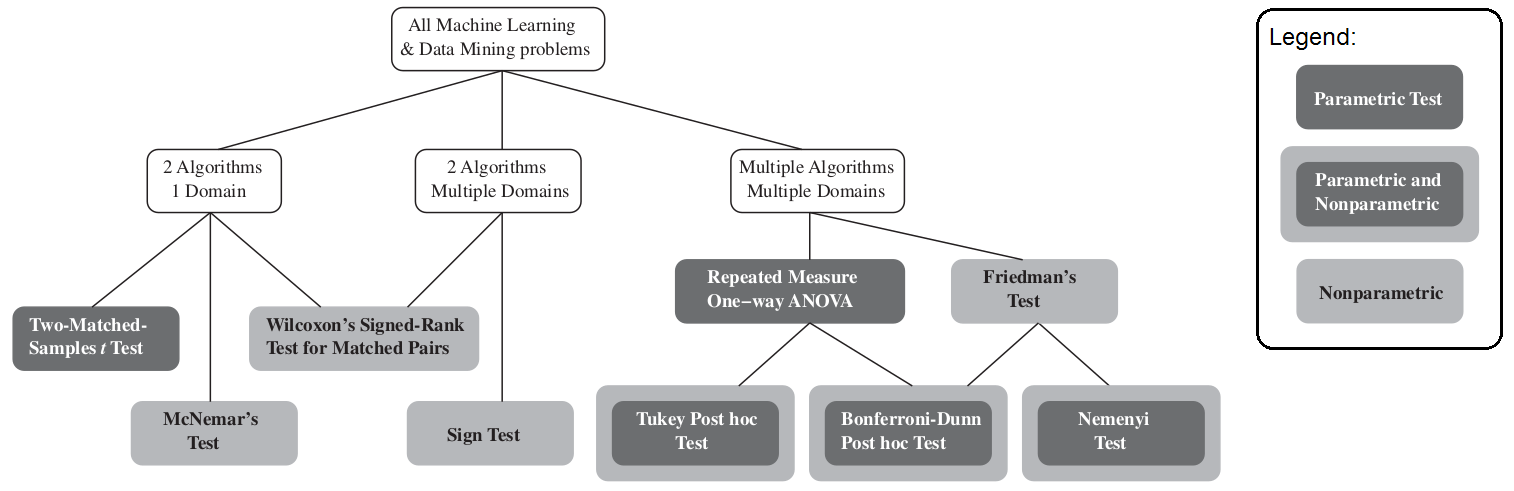
\includegraphics[width=\textwidth]{figure/tests_overview.png} \end{center}

% \footnotesize
% {\tiny{Source: \code{\url{https://marthawhite.github.io/mlcourse/lectures/2017/Lec20-MeasuringPerformance.pdf}}, p. 142.}\par}


% \end{frame}

\section{Scenario 1: Two Trained Models on 1 Data Set}
\begin{frame}{First Benchmarking Scenario}
\vfill
\centering
\large{Two trained models on 1 data set}
    \begin{figure}
        
\includegraphics[width = 0.6\textwidth]{figure/2algos_1dataset.png}
    \end{figure}
\vfill
\end{frame}


% \begin{frame}{Two-matched-samples t-test}

% \begin{itemize}
%     \setlength\itemsep{1em}
%     \item The two-matched-samples t-test (i.e., a paired t-test) is the simplest hypothesis test if the aim is to compare two \textbf{models} on a single test set based on arbitrary performance measures.
%     \item Due to being a parametric test, several distributional assumptions must be made:

%     \begin{itemize}
%         \setlength\itemsep{1em}
%         \item \textbf{(Pseudo-)normality}, usually met when sample size > 30.
%         \item \textbf{i.i.d. samples}, usually met if the loss of individual observations from a single test set is considered. % (this assumption is violated in case of resampling as ). %difficult as data is often limited (assumption is violated in the case of resampling).
%         \item \textbf{Equal variances of populations}, can be investigated by plots.
%     \end{itemize}
% \end{itemize}



% \end{frame}

\begin{frame}{Two-matched-samples t-test}
    % In contrast, Raschka (2018) starts his overview with an unpaired T-Test (testing the difference of proportions)


    % A paired t-test to compare two different models $\fh_1$ and $\fh_2$ w.r.t. a performance measure calculated on a test set of size $n_{\text{test}}$:

    \begin{itemize}
        \item Given a holdout test set $\Dtest$, can we assume a difference in performance between $\fh_1$ and $\fh_2$ generalizes to other data?
        $$H_0: \GE(\fh_1, L, \Dtest) = \GE(\fh_2, L, \Dtest) \text{ vs. } H_1: \GE(\fh_1, L, \Dtest) \neq \GE(\fh_2, L, \Dtest)$$
        \item Test statistic:
            $$
            T_{\text{t-test}} = \sqrt{n_{test}} \frac{\bar{d}}{\sigma_{d}} \sim t(n_{test} - 1), \text{ with }
            \sigma_{d} = \sqrt{\frac{1}{n_{\text{test}} - 1}\sum_{i=1}^{n_{test}} \left(d_i - \bar{d} \right)^2}
        $$
        $$d_i = L(\yi, \fh_1 (\xi)) - L(\yi, \fh_2 (\xi))\qquad \bar{d} = \frac{1}{n_{test}} \sum\limits_{i=1}^{n_{test}} d_i \qquad (\xi, \yi) \in \Dtest$$
        \item The two-matched samples t-test (or paired t-test) has multiple requirements:
        \begin{enumerate}
            \item \textbf{Loss values need to be iid samples} %Samples need to be iid samples from the underlying population
            % Only the case for a hold-out set but not for CV as loss is based on models that use overlapping obs. across CV folds.%, which, for instance, is not the case for cross-validation.

            \item \textbf{(Pseudo-) normality of loss values:}
            Requires a minimum of $\approx$ 30 loss values or loss values following a normal distribution.
            \item \textbf{Equal variances:} Assumes equal variances of both populations. %(if not, apply Welch test).
        \end{enumerate}
    \end{itemize}
\end{frame}
% xx

% \begin{frame}{Two-matched-samples t-test}
%     % \textbf{Note}: Here, $d_i$ is the difference of the outer loss of individual observations from the test set between the two models to be compared.
%     %\textbf{Issue}: $\GEh{n} \left(\fh_A\right)$ and $ \GEh{n} \left(\fh_B\right)$ are not independent as they are calculated on the same test set.

%     \begin{itemize}
%         \setlength\itemsep{1em}
%     \item We could also use a \textbf{$k$-fold CV paired t-test} to compare two \textbf{training algorithms} (instead of two models) on a single dataset.
%     \item Instead of comparing the outer loss of individual observations we would then compare the individual generalization errors per CV fold (i.e., the generalization error of the $k$ prediction models induced by the learning algorithm in each CV fold).
%     %\item Instad of using the difference of the outer loss of individual observations
%     \item Although the test sets do not overlap, the performance differences are not independent across CV folds due to overlapping training sets (which violates the assumption of i.i.d. samples).
%     %However, the paired t-test is a parametric test and is not recommended in practice as the assumptions of the student's t-test are often violated.
%     %\item A probably better alternative is, therefore, the Friedman test.
%     \item To partly overcome the issue of overlapping training sets across folds, Dietterich (1998) \footnote{Dietterich (1998). Approximate statistical tests for comparing supervised classification learning algorithms.}suggests using 5 times 2-fold CV so that at least within each repetition neither the training nor the test sets overlap.
%     % footnotes do not work
%     \end{itemize}
% \vspace{2cm} {\scriptsize Dietterich (1998). Approximate statistical tests for comparing supervised classification learning algorithms.}
% \end{frame}





% \begin{frame}{Weakness of Paired T-Test}

% \begin{itemize}
%     \setlength\itemsep{2em}
%     \item \textbf{Commensurability:} One has to be able to compare the differences over the data
%     sets, thus if the used performance measures have different properties for different
%     tasks, this assumption might be violated.
%     \item \textbf{(Pseudo-) Normality:} The t-test requires that (performance) samples come from a normal distribution or a minimum of 30 samples.
%     \item \textbf{Outliers:} Extreme values might skew the statistics and thus decrease a tests
%     power.
% \end{itemize}

% \end{frame}

\begin{frame}{Two-Matched-Samples T-Test}
\begin{itemize}
    \item \textbf{Example:} We evaluate learners \texttt{classif.rpart} and \texttt{classif.ranger} on the binary classification task \texttt{kin8nm}.
    \item We use the Brier score as loss function:
    {
        \scriptsize
        % latex table generated in R 4.1.2 by xtable 1.8-4 package
% Tue Oct 17 09:46:12 2023
\begin{table}[ht]
\centering
\begin{tabular}{rlrrrrr}
  \hline
id & truth & rpart\_prob & ranger\_prob & rpart\_loss & ranger\_loss & diff\_loss \\
  \hline
    1 & P & 0.7823 & 0.7759 & 0.0474 & 0.0502 & -0.0028 \\
      2 & P & 0.7823 & 0.9432 & 0.0474 & 0.0032 & 0.0442 \\
      \vdots & \vdots & \vdots & \vdots & \vdots & \vdots & \vdots \\
   8192 & P & 0.4489 & 0.8476 & 0.3038 & 0.0232 & 0.2805 \\
   \hline
\end{tabular}
\end{table}

    }
    \item The test statistic corresponds to:
    $$
    T_{\text{t-test}} = \sqrt{8192} \; \frac{0.0016}{0.178} = 79.523
    $$
    \item For $\alpha = 0.05$, the critical values to reject $H_0$ are -1.9637 and 1.9637.
    \item For the given significance level, there is enough evidence to reject $H_0$. We assume the is a difference in performance on this population of data.
\end{itemize}

\end{frame}


\begin{frame}{McNemar Test for Classification}
% https://slideplayer.com/slide/9574350/
\begin{itemize}
% \item The McNemar test compares the relative errors of two models.
\item McNemar test is non-parametric (no distributional assumptions).
\item Caveat: Only works for classification tasks.
\item $H_0$: $(A + B = A + C) \land (C + D = B + D) \Rightarrow H_0: B = C \text{ vs. } H_1$:  $B \neq C$
\item Test statistic:
$$T_{\text{McNemar}} =  \tfrac{(|B-C| - 1)^2}{B + C} \sim \chi^2_{1}
$$
% when the considered performance measure is based on an outer loss with a nominal or binary output, e.g., accuracy is based on a binary outer loss.
% \item Both models are trained on a training set and evaluated on a test set. Based on the test set, a \textbf{contingency table} that compares the two models (model 1 and model 2) is calculated:
\end{itemize}

\begin{minipage}{0.45\textwidth}
\includegraphics[width=\textwidth]{figure/mcnemar_1.png} \end{minipage}
\begin{minipage}{0.54\textwidth}
\begin{itemize}
\item A: $\#$ obs. correctly classified by both.
\item B: $\#$ obs. misclassified by model 2 but not by model 1.
\item C: $\#$ obs. misclassified by model 1 but not by model 2.
\item D: $\#$ obs. misclassified by both.
\end{itemize}
\end{minipage}
\end{frame}

% \begin{frame}{McNemar Test}

% \begin{minipage}[c]{0.4\linewidth}
%   \begin{center}
%   \renewcommand{\arraystretch}{1.5}
%   \begin{tabular}{cc|cc}
%       & & \multicolumn{2}{c}{$f_2$} \\
%       & & $0$ & $1$ \\
%       \hline
%       \multirow{2}{*}{ $f_1$} & $0$ & $c_{00}^{Mc}$ & $c_{01}^{Mc}$ \\
%       & $1$ & $c_{10}^{Mc}$ & $c_{11}^{Mc}$ \\
%   \end{tabular}
%   \end{center}
% \end{minipage} % no space if you would like to put them side by side
% \begin{minipage}[c]{0.59\linewidth}
% \vspace{0.15cm}
%   $c_{00}^{Mc} = \sum_{i=1}^{|S_{test}|} \left[ I(f_1(\mathbf{x_i}) \neq y_i) \wedge I(f_2(\mathbf{x_i}) \neq y_i) \right]$ \vspace{0.05cm}

%   $c_{01}^{Mc} = \sum_{i=1}^{|S_{test}|} \left[ I(f_1(\mathbf{x_i}) \neq y_i) \wedge I(f_2(\mathbf{x_i}) = y_i)\right]$ \vspace{0.05cm}

%   $c_{10}^{Mc} = \sum_{i=1}^{|S_{test}|} \left[ I(f_1(\mathbf{x_i}) = y_i) \wedge I(f_2(\mathbf{x_i}) \neq y_i)\right]$ \vspace{0.05cm}

%   $c_{11}^{Mc} = \sum_{i=1}^{|S_{test}|} \left[ I(f_1(\mathbf{x_i}) = y_i) \wedge I(f_2(\mathbf{x_i}) = y_i)\right]$

% \end{minipage}
% \vspace{0.5cm}

% Testing: $H_0$: $c_{01}^{Mc} = c_{01}^{Mc} = c_{null}^{Mc}$

% $$\chi^2_{Mc} =  \frac{(|c_{01}^{Mc} - c_{01}^{Mc}| - 1)^2}{c_{01}^{Mc} + c_{10}^{Mc}} \overset{approx}{\sim} \chi^2_{1,1-\alpha}$$

% If $c_{01}^{Mc} + c_{01}^{Mc} < 20$, approximation doesn't work, use binomial instead

% \end{frame}

% \begin{frame}{McNemar Test}


% \begin{minipage}[c]{0.625\linewidth}
% Given such a contingency table, the accuracy of each model can be computed as follows:
% \begin{itemize}
%   \item Model 1: (A+B)/(A+B+C+D)
%   \item Model 2: (A+C)/(A+B+C+D)
% \end{itemize}

% Even if the models have \textbf{equal} accuracy (indicating equal performance), cells B and C may differ because the models may misclassify different instances.
% \end{minipage}
% % \begin{minipage}[c]{0.365\linewidth}
% %   \includegraphics{figure_man/mcnemar_1.png}
% % \end{minipage}

% \lz McNemar tests the following hypotheses:
% \begin{itemize}
% \item $H_0:$ Both models have the same performance (we expect B = C).
% \item $H_1:$ Performances of the two models are not equal.
% \end{itemize}
% %\lz
% The test statistic is computed by
% $$\chi^2_{Mc} =  \tfrac{(|B-C| - 1)^2}{B + C} \sim \chi^2_{1}.$$

% \textbf{Note}: The McNemar test should only be used if $B + C > 20$.
% \end{frame}

% \begin{frame}{McNemar's Test for Classifiers}

% \begin{itemize}
%     % \setlength\itemsep{1em}
%     \item McNemar's test compares the errors of two models in a 2x2 contingency matrix:
%     \begin{figure}
%         \centering
%         \includegraphics[width = 0.6\textwidth]{mcnemar_contingency_table_ex1.png}
%         \label{fig:enter-label}
%     \end{figure}
%     \item Both models seem to perform equally well (model 1 accuracy: 9,960 / 10,000 = 99.6\%; model 2 accuracy: 9,970 / 10,000 = 99.7\%).
%     \item In subfigure A, model 2 got 11 predictions right that model 1 got wrong; model 2 got 1 prediction right that model 2 got wrong (ratio 11:1).
%     $\Rightarrow$ Model 2 seems to perform better than model 1.
%     \item In subfigure B, the ratio is 25:15, which makes it less clear to choose a better-performing model.
% \end{itemize}

% \end{frame}


% \begin{frame}{McNemar's Test for Classifiers}

% \begin{itemize}
%     % \setlength\itemsep{1em}
%     \item This relative error rate of two models can be used for a statistical test.
% \end{itemize}

% \end{frame}

\begin{frame}{McNemar Test}

% The test statistic is computed by
% $$\chi^2_{Mc} =  \tfrac{(|B-C| - 1)^2}{B + C} \sim \chi^2_{1}.$$
\textbf{Continuing previous example}:

\begin{center}
  %\renewcommand{\arraystretch}{1.5}
%\hspace*{\fill}
  \begin{tabular}{cc|cc}
      & & \multicolumn{2}{c}{\textbf{ranger}} \\
      & & correct & wrong \\
      \hline
      \multirow{2}{*}{\textbf{rpart}} & correct & 5942 & 1 \\
      & wrong & 2232 & 17 \\
  \end{tabular}
\end{center}

Calculate the test statistic:

$$T_{\text{McNemar}} =  \frac{(|1 - 2232| - 1)^2}{1 + 2232} \approx 2227
$$
% > 3.841 = \chi^2_{1,0.95}.$$
\begin{itemize}
    \item For $\alpha = 0.5$, the critical value is 3.841.
    \item $T_{\text{McNemar}} > 3.841 \Rightarrow$ Reject $H_0$.
    \item We conclude that the tree and random forest do not have the same performance on this population of data.
    \item The t-test performs on observation-wise loss values, while the McNemar test performs on aggregate classification errors.
\end{itemize}
% We can reject $H_0$ at a significance level of 0.05, i.e., we reject the hypothesis that the tree and the random forest have the same performance.
% and assume that our tree and our random forest classify the data differently

\end{frame}


% \begin{frame}{McNemar Test}

% \begin{itemize}
% \item McNemar test is a non-parametric test that compares the errors of two classifiers.
% \item classifiers have to be trained and tested on the same dataset.
% % \item $H_0$: the two classifiers have the same error rates, \\ $H_1$: the error rates differ
% \item Goodness-of-fit measure: Compares observed counts with expected distribution under $H_0$.
% \item Relies on contingency matrix and is very similar to $\chi^2$-Test.
% \item McNemar test considers if observations are classified correctly or not and does not provide any quantification of these measures.
% \item According Dietterich(1998), the McNemar test should only be used if $B + C > 20$.
% \end{itemize}
% %

% \end{frame}

%  \begin{frame}{T-test vs. McNemar Test}

% Apart from t-test being parametric and the McNemar test being non-parametric, two tests have other significant differences. Because of its nature, it is possible to construct intervals for t-test however it is not possible to work with intervals for McNemar test which only works with nominal performance measures. McNemar test takes into account that whether observations are classified correctly or not and it does not provide any quantification of these measures.

% \lz

% According to the Dietterich(1998), one can proceed with McNemar test when the number of disagreement between two classifiers $c_{01}^{Mc} + c_{01}^{Mc} $ is greater than 20.

% \end{frame}

% The following compares the performance of multiple classifiers on one datasets
% \begin{frame}{Cochran's Q Test? (not a slide)}

%     \begin{itemize}
%         \item Generalization of McNemar test to 3 or more models.
%         \item Not as good as Friedman or Nemeniy?
%     \end{itemize}
% \end{frame}


\section{Scenario 2: Two Algorithms on Multiple Data Sets}
\begin{frame}{Second Benchmarking Scenario}
% https://docs.google.com/presentation/d/1hRPhxdXPvF2J2xXR_aDiG4Y3GxvMbNvujkPuJ-tsHRY/edit?usp=sharing
\vfill
\centering
\large{Two algorithms on multiple data sets}
    \begin{figure}
        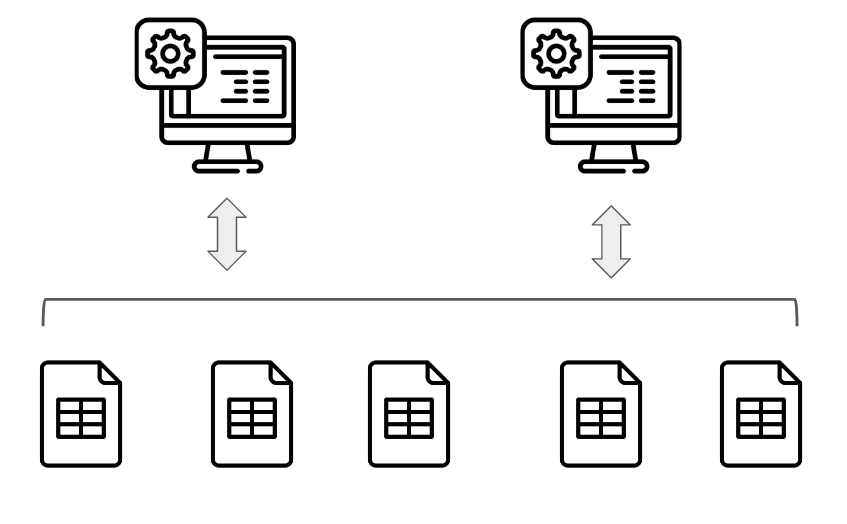
\includegraphics[width = 0.6\textwidth]{figure/2algos_multipledatasets.png}
    \end{figure}
\vfill
\end{frame}

\begin{frame}{Wilcoxon Signed Rank Test}
    \begin{itemize}
        % \item The Wilcoxon signed rank test ranks differences in performance of two classifiers, ignores the signs, and then compares ranks for positive and negative differences.
        \item Non-parametric and suitable for any performance measure.
        \item $H_0$: Algs. 1 and 2 have tied ranks in model performance. \\
        $H_1$: Algs. 1 and 2 have different ranks in performance.
        \item Consider $M$ data sets with performance $\widehat{\text{GE}}(\widehat{f}_k, \rho, \Dtestm)$ for model $k$ and data set $m$. The difference $d_m$ between GE estimates on the $m$-th data set is:
        $$
        d_m = \widehat{\text{GE}}(\widehat{f}_1, \rho, \Dtestm) - \widehat{\text{GE}}(\widehat{f}_2, \rho, \Dtestm)
        $$
        \item Let $R^{+}$ denote the rank sum of absolute differences $|d_m|$ for data sets where algorithm 1 outperforms algorithm 2 and vice versa for $R^{-}$. Ranks of $d_m = 0$ are split evenly among the sums (if there is an odd number of them, one is ignored):
        $$
        R^{+} = \sum_{d_m > 0} \text{rank}(|d_m|) + \frac{1}{2} \sum_{d_m = 0} \text{rank}(|d_m|) \quad\quad R^{-} = \sum_{d_m < 0} \text{rank}(|d_m|) + \frac{1}{2} \sum_{d_m = 0} \text{rank}(|d_m|)
        $$
        \item The test statistic does not follow a closed-form distribution, but probabilities can be derived from a distribution table:
        $$
        T_{\text{Wilcoxon}} = \frac{\min(R^{+}, R^{-})   - \frac{1}{4}M(M + 1)}{\sqrt{\frac{1}{24}M(M + 1)(2M + 1)}}
        $$
    \end{itemize}
\end{frame}


\begin{frame}{Wilcoxon Signed Rank Test}
    \begin{itemize}
        \item A benchmark of rpart and ranger (with default hyperparameters) on 6 classification tasks, using the classification error as performance measure:
    {
        \scriptsize
        % latex table generated in R 4.3.3 by xtable 1.8-4 package
% Mon Nov 18 17:21:35 2024
\begin{table}[ht]
\centering
\begin{tabular}{rlrrrr}
  \hline
 & task\_id & rpart & ranger & diff & rank \\ 
  \hline
1 & pollen & 0.4987 & 0.5005 & -0.0018 &     2 \\ 
  2 & threeOf9 & 0.1543 & 0.0117 & 0.1426 &     6 \\ 
  3 & fri\_c1\_500\_5 & 0.1900 & 0.1180 & 0.0720 &     4 \\ 
  4 & space\_ga & 0.2240 & 0.1629 & 0.0611 &     3 \\ 
  5 & kin8nm & 0.2795 & 0.1608 & 0.1187 &     5 \\ 
  6 & monks-problems-3 & 0.0108 & 0.0108 & 0.0000 &     1 \\ 
   \hline
\end{tabular}
\end{table}

    }
% https://edisciplinas.usp.br/pluginfile.php/4129451/mod_resource/content/1/model_selection_evaluation.pdf
% \textbf{Example:} AUC of two algorithms on multiple data sets

% \begin{table}[!ht]
%     \scriptsize
%     \centering
%     \begin{tabular}{|l|l|l|}
%     \hline
%         \textbf{data set} & \textbf{algorithm 1} & \textbf{algorithm 2} \\ \hline\hline
%         adult & 0.763 & \textbf{0.768} \\ \hline
%         % breast\_cancer & 0.599 & 0.591 & \\ \hline
%         breast\_cancer\_wisconsin & 0.954 & \textbf{0.971} \\ \hline
%         % cmc & 0.628 & 0.661 & \\ \hline
%         ionosphere & 0.882 & \textbf{0.888} \\ \hline
%         % iris & 0.936 & 0.931 & \\ \hline
%         % liver\_disorders & 0.661 & 0.668 & \\ \hline
%         lung\_cancer & \textbf{0.583} & \textbf{0.583} \\ \hline
%         % lymphography & 0.775 & 0.838 & \\ \hline
%         mushroom & \textbf{1.000} & \textbf{1.000} \\ \hline
%         % primary\_tumor & 0.940 & 0.962 & \\ \hline
%         % rheum & 0.619 & 0.666 & \\ \hline
%         % voting & 0.972 & 0.981 & \\ \hline
%         wine & 0.957 & \textbf{0.978} \\ \hline
%     \end{tabular}
% \end{table}
$$
    R^{+} = 2\qquad R^{-} = 15\qquad \min(R^{+}, R^{-}) = 2
    $$
    $$
    T_{\text{Wilcoxon}} = \frac{2 - \frac{1}{4}6(6 + 1)}{\sqrt{\frac{1}{24}6(6 + 1)(12 + 1)}} = - 1.78
    $$
    \item For $\alpha = 0.05$, the critical value (two-sided) is 1.
    \item $T_{\text{Wilcoxon}} < 1 \Rightarrow$ reject $H_0$!
    \item There is evidence that the two algorithms do not perform equally well.
\end{itemize}

\end{frame}

\begin{frame}{Further notes}
    \vfill
    \begin{itemize}
        \item Wilcoxon Signed Rank Test assumes commensurability of scores $\rightarrow{}$ use sign test if violated
        \item Researchers use the Wilcoxon Signed Rank Test to compare two algorithms on the same data, but violate independence assumption
    \end{itemize}
    \vfill
\end{frame}

%\section{Scenario 2: Two Algorithms on One Data Set}
%\begin{frame}{Second Benchmarking Scenario}
%% https://docs.google.com/presentation/d/1hRPhxdXPvF2J2xXR_aDiG4Y3GxvMbNvujkPuJ-tsHRY/edit?usp=sharing
%\vfill
%\centering
%\large{Two algorithms on 1 data set}
%    \begin{figure}
%        
\includegraphics[width = 0.6\textwidth]{figure/2algos_1dataset.png}
%    \end{figure}
%\vfill
%\end{frame}


\section{Scenario 3: Multiple Algorithms on Multiple Data Sets}
\begin{frame}{Third Benchmarking Scenario}
% https://docs.google.com/presentation/d/1hRPhxdXPvF2J2xXR_aDiG4Y3GxvMbNvujkPuJ-tsHRY/edit?usp=sharing
\vfill
\centering
\large{Multiple algorithms on multiple data sets}
    \begin{figure}
        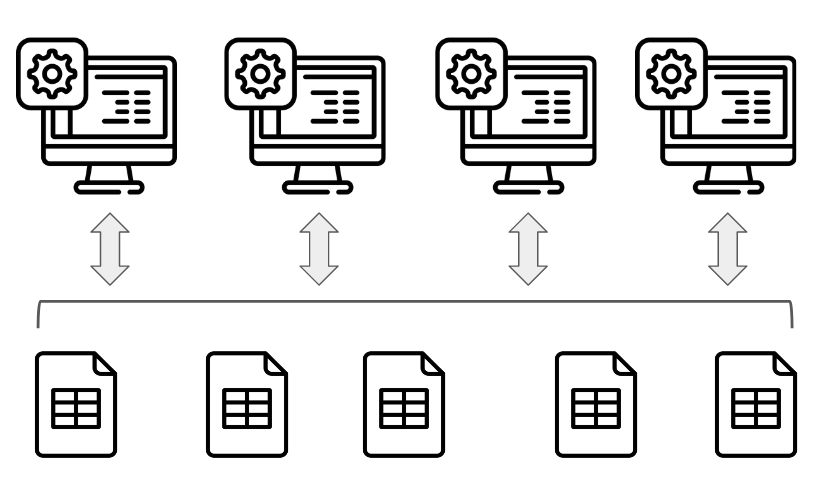
\includegraphics[width = 0.6\textwidth]{figure/multiplalgos_multipledatasets.png}
    \end{figure}
\vfill
\end{frame}

\begin{frame}{Comparing Multiple Models}

\begin{itemize}
    \setlength\itemsep{1em}
    \item So far: comparing perf. of 2 models
    \item Now: comparing multiple models using omnibus test
    %So far, we have only been comparing the performance of two models. When comparing multiple models, we can make use of an omnibus test.
    \item Omnibus hypotheses to be tested are:
        \begin{itemize}
            \item $H_0:$ All algorithms are equivalent in their performance and hence their average ranks should be equal.
            \item $H_1:$ The average rank for at least one algorithm is different.
        \end{itemize}
    \item Omnibus tests are only useful to indicate that at least one model performs differently than the others.\\
    $\Rightarrow$ If yes, run post-hoc pairwise comparisons.
    % \item We first run an omnibus Friedman test, and if if $H_0$ is rejected, we run pairwise comparisons via the post-hoc Nemenyi test or the post-hoc Bonferroni-Dunn test.
\end{itemize}

\begin{figure}
    \centering
    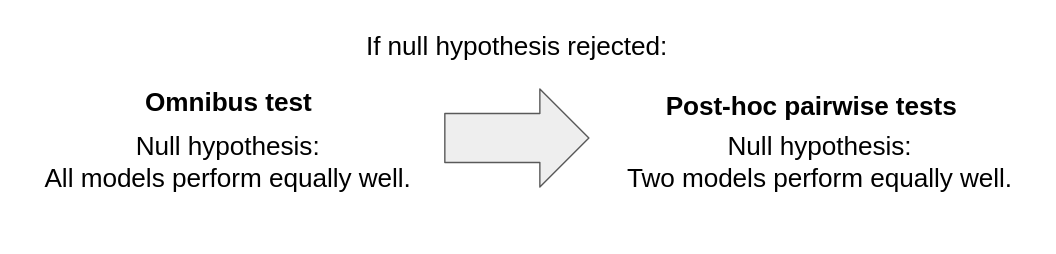
\includegraphics{figure/omnibustesting.png}
    % \caption{Caption}
    % \label{fig:enter-label}
\end{figure}

\end{frame}

%\section{Compare Multiple Models Multiple Domains}

\begin{frame}{Friedman Test}

\begin{itemize}
\item Example of a benchmark of 6 mlr3 learners (with default hyperparameters) on 16 classification tasks, using the classification error as performance measure:

\end{itemize}
% \textbf{Illustrative example ($M < 15$ and $K < 5$ here, so test statistic not $\chi^2$-distributed):}

    % \begin{table}[!ht]
    %     \scriptsize
    %     \centering
    %     \begin{tabular}{|l|l|l|l|l|}
    %     \hline
    %         \textbf{data set} & \textbf{algorithm 1} & \textbf{algorithm 2}  & \textbf{algorithm 3} & \textbf{algorithm 4} \\ \hline\hline
    %         adult & 0.763 (4) & 0.768 (3) & 0.771 (2) & 0.798 (1) \\ \hline
    %         % breast\_cancer & 0.599 & 0.591 & \\ \hline
    %         breast\_cancer\_wisconsin & 0.954 (4) & 0.971 (1) & 0.968 (2) & 0.967 (3) \\ \hline
    %         % cmc & 0.628 & 0.661 & \\ \hline
    %         ionosphere & 0.882 (4) & 0.888 (2) & 0.886 (3) & 0.898 (1) \\ \hline
    %         % iris & 0.936 & 0.931 & \\ \hline
    %         % liver\_disorders & 0.661 & 0.668 & \\ \hline
    %         lung\_cancer & 0.583 (2.5) & 0.583 (2.5) & 0.563 (4) & 0.625 (1) \\ \hline
    %         % lymphography & 0.775 & 0.838 & \\ \hline
    %         mushroom & 1.000 (2.5) & 1.000 (2.5) & 1.000 (2.5) & 1.000 (2.5) \\ \hline
    %         % primary\_tumor & 0.940 & 0.962 & \\ \hline
    %         % rheum & 0.619 & 0.666 & \\ \hline
    %         % voting & 0.972 & 0.981 & \\ \hline
    %         wine & 0.957 (3) & 0.978 (1) & 0.946 (4) & 0.970 (2) \\ \hline
    %     \end{tabular}
    % \end{table}
% \begin{align*}
%     \bar{R} &= \frac{1}{6 \cdot 4} \sum_{k=1}^{4} \sum_{m=1}^{6} R_{mk} = \frac{60}{24} = 2.5 \\
%     SS_{Total} &= 6 \sum_{k=1}^{4} (\bar{R}_{.k} - 2.5)^2 = 6 \cdot \left(3.333^2 + 2^2 + 2.916^2 + 1.75^2 \right) \approx 160.047
%     % , where \bar{R}_{.k} =  \frac{1}{B} \sum_{b=1}^{B} R_{bk}
%     \\
%     SS_{Error} &= \frac{1}{6(4-1)} \sum_{m=1}^{6} \sum_{k=1}^{4} (R_{mk} - \bar{R})^2 = 1.375 \\
%     T_{\text{Friedman}} &= \frac{SS_{Total}}{SS_{Error}} = \frac{160.047}{1.375} \approx 116.4 > 7.815 \Rightarrow \text{Reject $H_0$!}
% \end{align*}

{
    \tiny
    % latex table generated in R 4.1.2 by xtable 1.8-4 package
% Tue Oct 10 14:57:30 2023
\begin{table}[ht]
\centering
\begin{tabular}{rlllllll}
  \hline
 & task\_id & featureless & cv\_glmnet & rpart & ranger & kknn & svm \\
  \hline
1 & pollen & 0.5148 (5.5) & 0.5148 (5.5) & 0.4987 (1) & 0.5005 (2) & 0.5107 (4) & 0.5013 (3) \\
  2 & threeOf9 & 0.4648 (6) & 0.2228 (5) & 0.1543 (4) & 0.0117 (2) & 0.1231 (3) & 0.0078 (1) \\
  \vdots & \vdots & \vdots & \vdots & \vdots & \vdots & \vdots & \vdots \\
 16 & strikes & 0.5312 (6) & 0.4016 (5) & 0.0993 (2) & 0.0288 (1) & 0.1184 (3) & 0.2528 (4) \\
   \hline
\end{tabular}
\end{table}

}
    \centering
    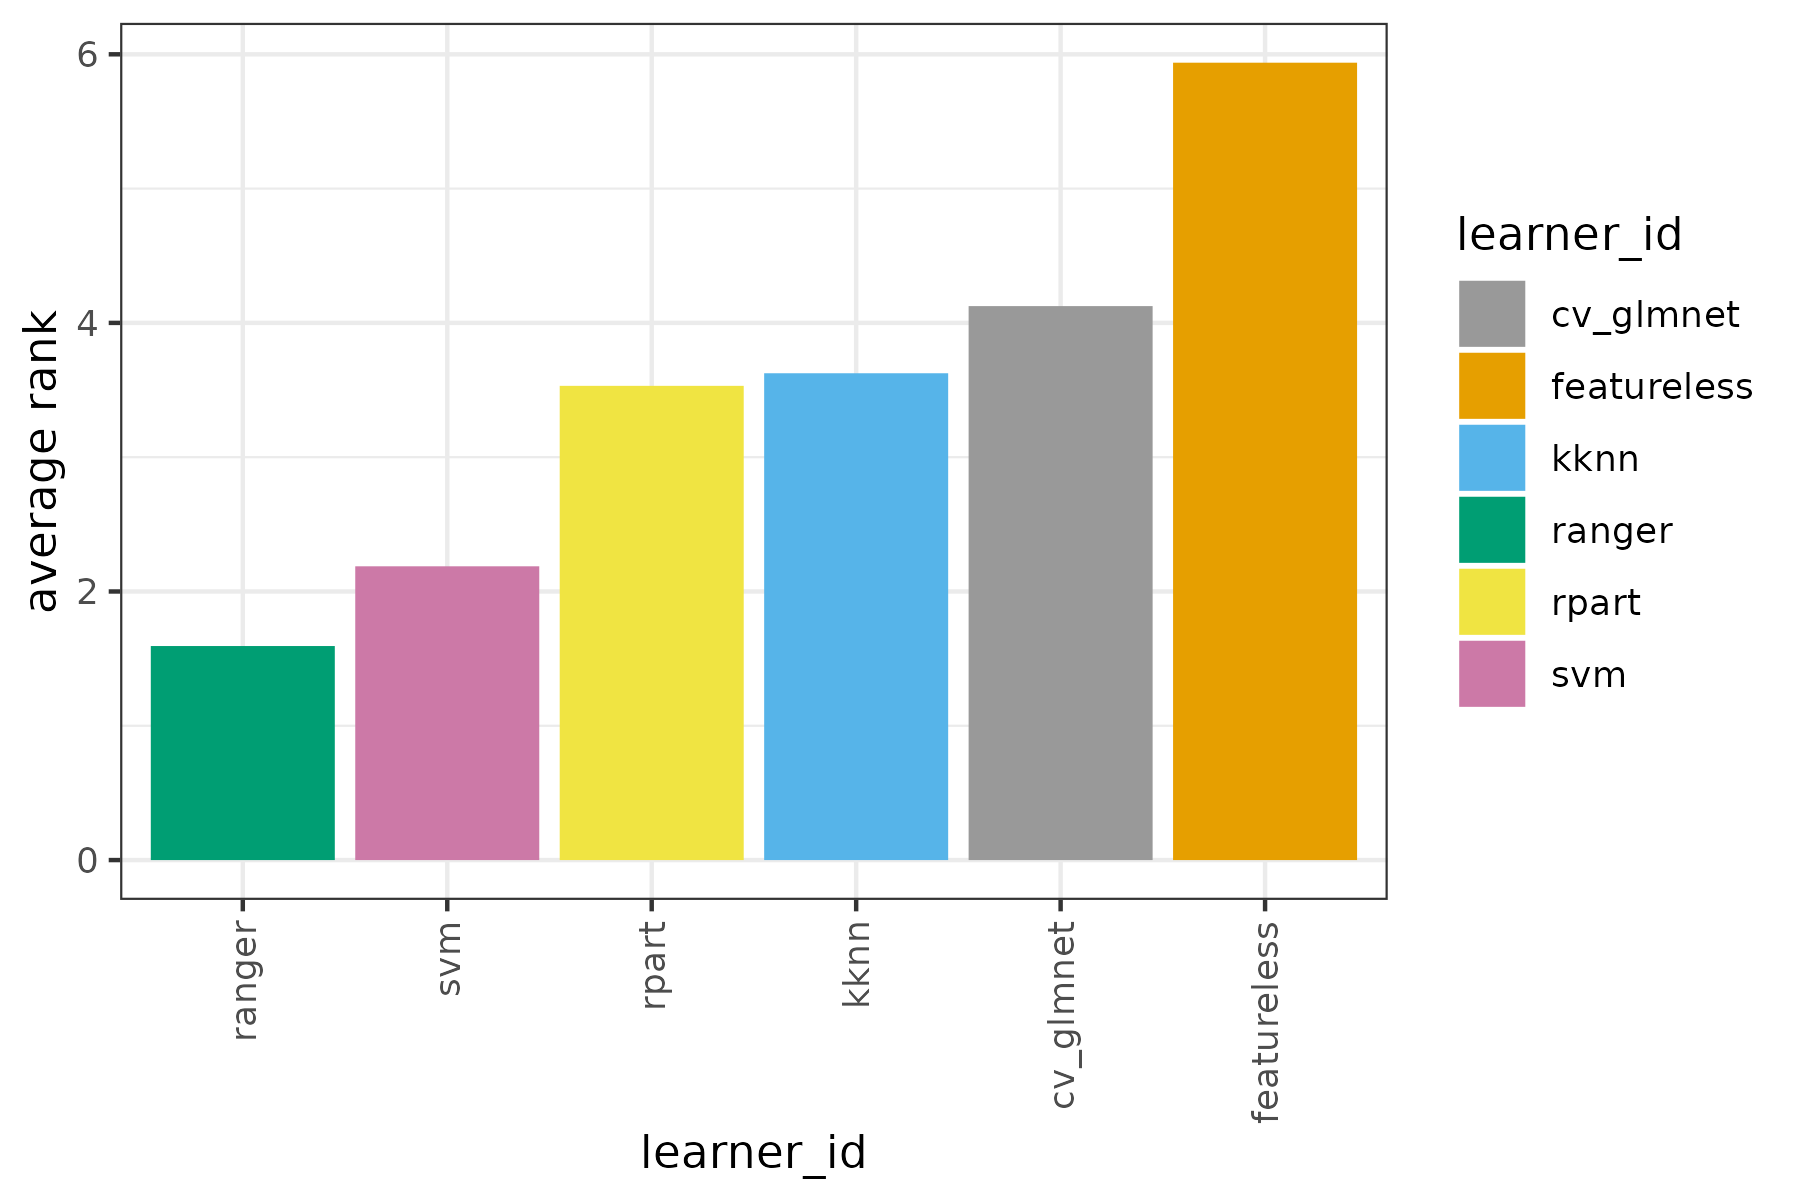
\includegraphics[width = 0.65\textwidth]{figure/benchmarkrankplot.png}

\end{frame}

% \begin{frame}{Friedman test}
%     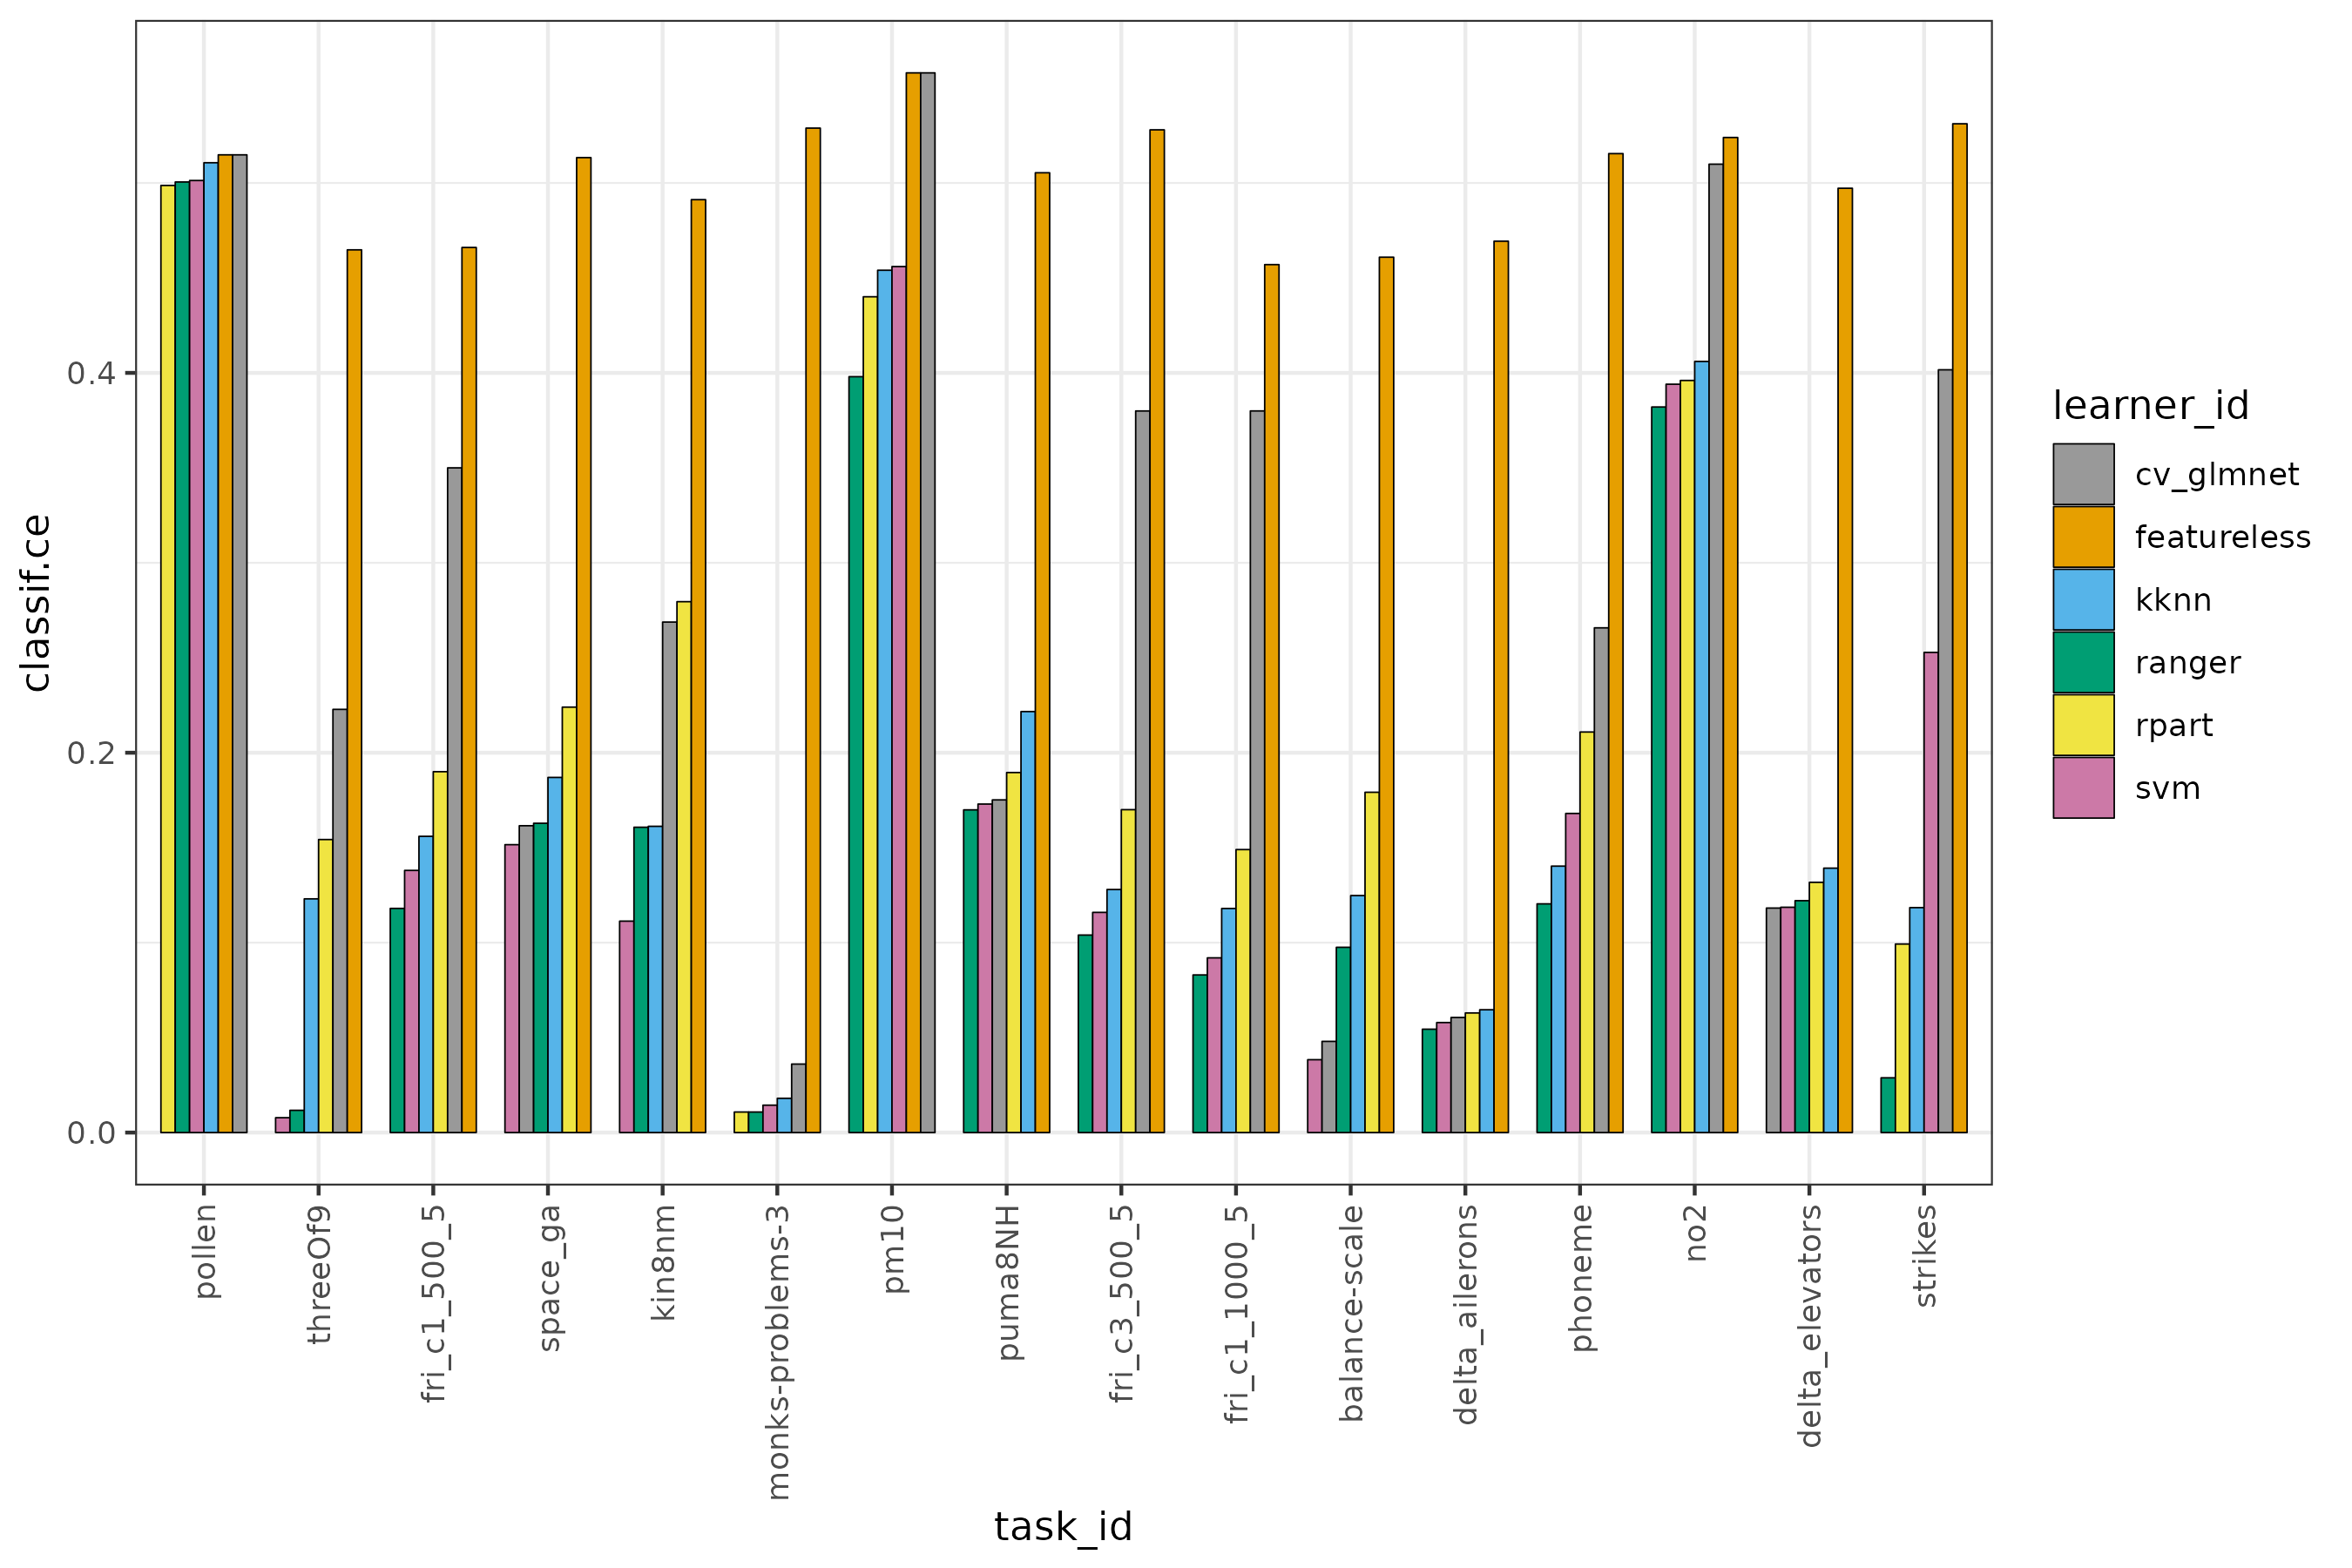
\includegraphics[width = \textwidth]{figure/benchmarkcolplot.png}
% \end{frame}

% \begin{frame}{Friedman test}
%     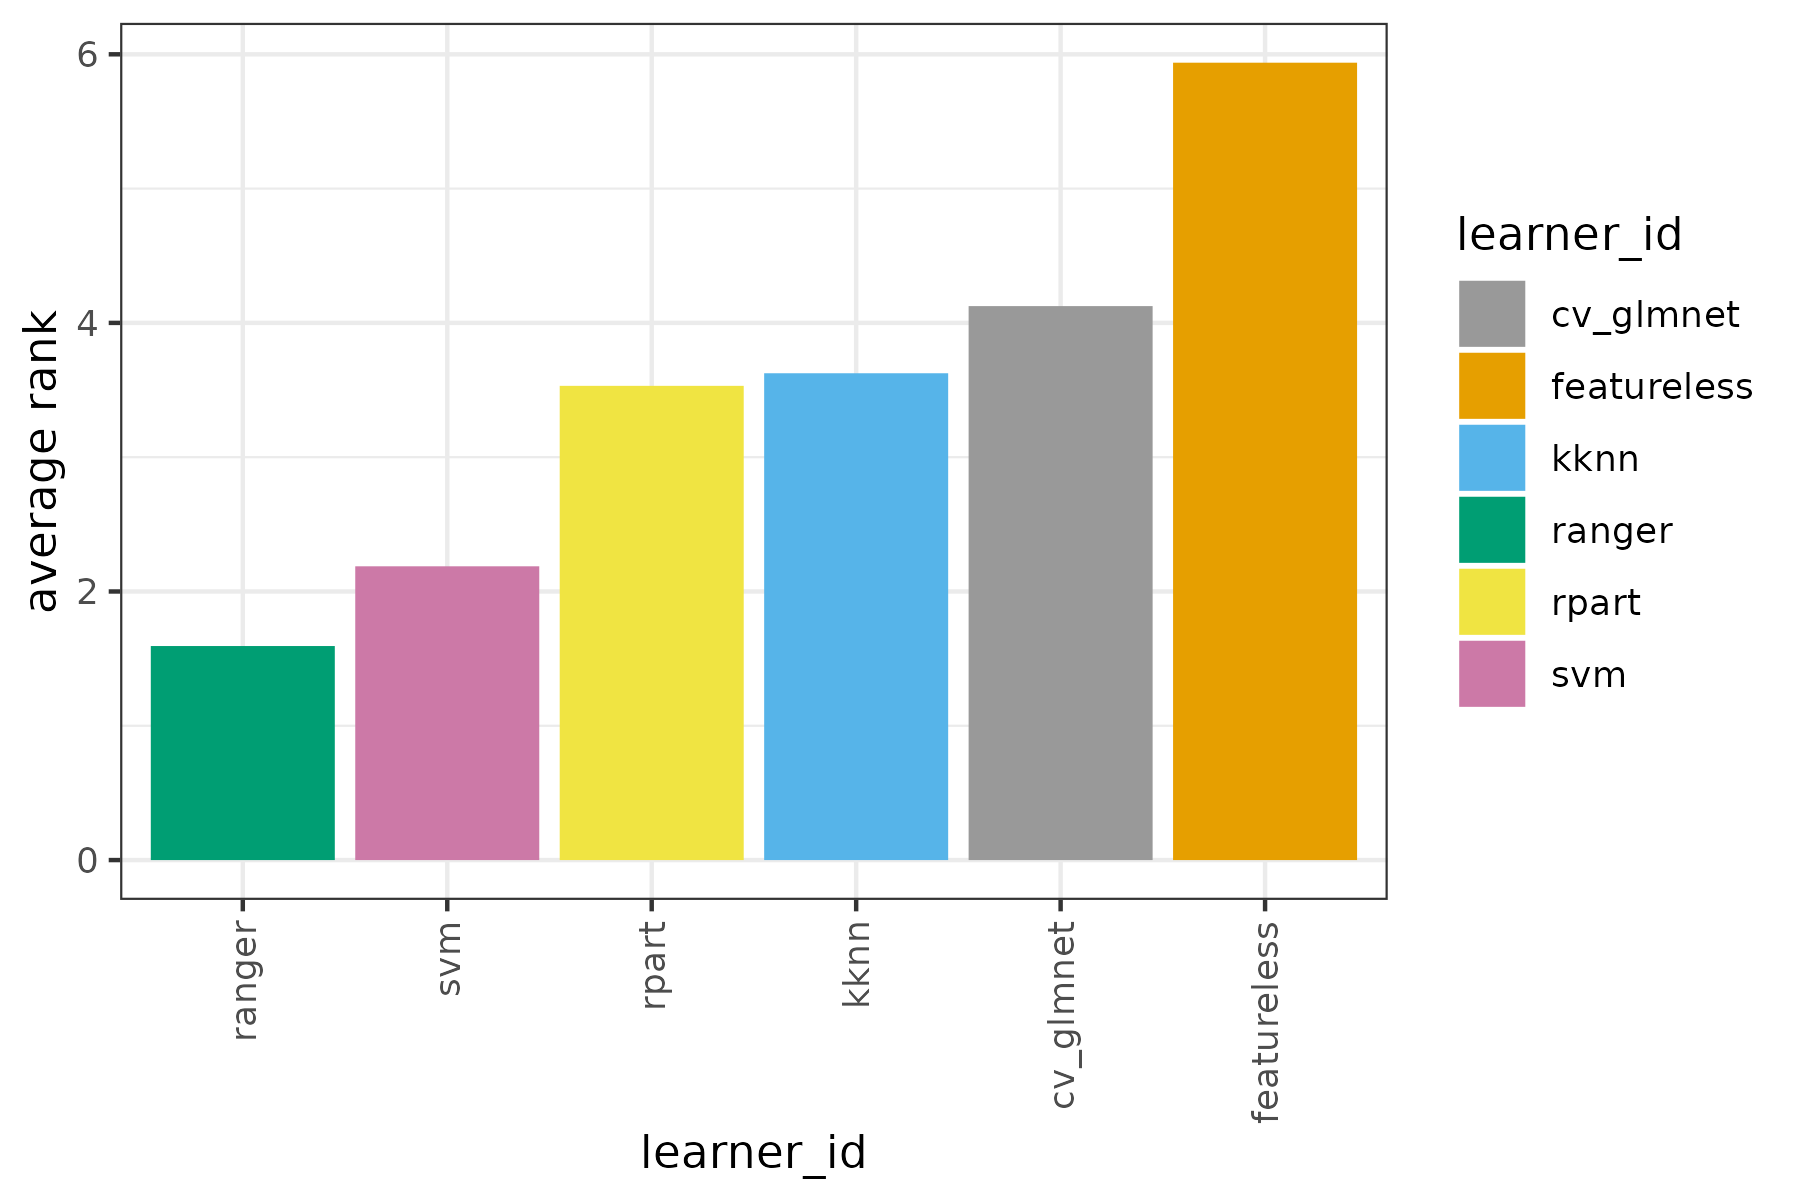
\includegraphics[width = 0.5\textwidth]{figure/benchmarkrankplot.png}
% \end{frame}


% Suppose we want to evaluate $M$ data sets and K$ algorithms. The Friedman test first ranks algorithms for each data set separately:

% \begin{itemize}
%   \item Separately rank each algorithm for each dataset from best-performing (lowest rank) to worst-performing (highest rank), using any performance measure.
%   \item If there is a $d$-way tie after rank $r$, assign a rank of $ \left[(r+1) + (r+2) + ... + (r+d)\right] /d $ to all tied classifiers.
%   \item Let $R_{mk}$ denote the rank of algorithm $k$ on data set $m$.
% \end{itemize}

\begin{frame}{Friedman Test}

After ranking algorithms, we calculate the following quantities (where $M$ denotes the number of data sets and $K$ the number of algorithms):

\begin{itemize}
  \item The overall mean rank:
  \begin{flalign*}
     & \bar{R} = \frac{1}{mk} \sum_{k=1}^{K} \sum_{m=1}^{M} R_{mk}
      = \frac{1}{96} \sum_{k=1}^{6} \sum_{m=1}^{16} R_{mk} = 3.5 &
  \end{flalign*}
  \item The total sum of squares:
  \begin{flalign*}
    & SS_{Total} = M \sum_{k=1}^{K} (\bar{R}_{.k} - \bar{R})^2 = 16 \sum_{k=1}^{6} (\bar{R}_{.k} - 3.427)^2 \approx 187.281 & \\
  & \text{with the mean rank for the $k$-th algorithm } \bar{R}_{.k} = \frac{1}{M} \sum_{m=1}^{M} R_{mk} = \frac{1}{16} \sum_{m=1}^{16} R_{mk} &
  \end{flalign*}
  \item The error sum of squares:
    \begin{flalign*}
        & SS_{Error} = \frac{1}{M(K-1)} \sum_{m=1}^{M} \sum_{k=1}^{K} (R_{mk} - \bar{R})^2 = \frac{1}{80} \sum_{m=1}^{16} \sum_{k=1}^{6} (R_{mk} - 3.427)^2\approx 3.481 &
    \end{flalign*}
\end{itemize}

\end{frame}

\begin{frame}{Friedman Test}

\begin{itemize}
\itemsep2em
\item The Friedman test statistic is calculated as:

$$T_{\text{Friedman}} = \frac{SS_{Total}}{SS_{Error}} \approx 52.872
$$
\item For sufficiently large \textit{M} ($>15$) and \textit{K} ($>5$): $$
T_{\text{Friedman}} \sim \chi_{K-1}^2
$$
\item The  $(1-\alpha)$ quantile of $\chi_{5}^2$ corresponds to 11.075, leading us to reject $H_0$.
\item We assume there is at least one algorithm performing better than the remaining algorithms. Which one(s) needs to be determined with pairwise post-hoc tests.

\end{itemize}

\end{frame}


% \begin{frame}{Friedman test}
% % So far we have only compared 2 models / algorithms on one dataset. The \textbf{Friedman test} can be used to compare multiple classifiers on multiple datasets. The hypotheses to be tested are:
% % \begin{itemize}
% % \item $H_0:$ All algorithms are equivalent in their performance and hence their average ranks should be equal.
% % \item $H_1:$ The average rank for at least one algorithm is different.
% % \end{itemize}

% Suppose we want to evaluate $m$ data sets and $k$ algorithms. The Friedman test first ranks algorithms for each data set separately:

% \begin{itemize}
%   \item Separately rank each algorithm for each dataset from best-performing to worst-performing, using any performance measure of interest.
%   \item If there is a $d$-way tie after rank $r$, assign a rank of $ \left[(r+1) + (r+2) + ... + (r+d)\right] /d $ to all tied classifiers.
%   \item Let $R_{ij}$ denote the rank of algorithm $j$ on data set $i$.
% \end{itemize}

% After ranking algorithms, calculate the following quantities:

% \begin{itemize}
%   \item The overall mean rank:
%   $ \bar{R} = \frac{1}{mk} \sum_{i=1}^{m} \sum_{j=1}^{k} R_{ij}. $
%   \item The total sum of squares:
%   $ SS_{Total} = m \sum_{j=1}^{k} (\bar{R}_{.j} - \bar{R})^2 $, where $\bar{R}_{.j} =  \frac{1}{m} \sum_{i=1}^{m} R_{ij}$.
%   \item The error sum of squares:
%   $ SS_{Error} = \frac{1}{m(k-1)} \sum_{i=1}^{m} \sum_{j=1}^{k} (R_{ij} - \bar{R})^2. $
% \end{itemize}

% The Friedman test statistic is calculated as:

% $${\chi_F}^2 = \frac{SS_{Total}}{SS_{Error}} \sim \chi_{k-1}^2 \text{ for large \textit{m} ($>15$) and \textit{k} ($>5$).}$$
% \end{frame}



% \begin{frame}{Friedman test}
% After obtaining the rank for each algorithm $j$ on different datasets $i$, calculate the following quantities:

% \begin{itemize}
%   \item The overall mean rank:
%   $ \bar{R} = \frac{1}{mk} \sum_{i=1}^{m} \sum_{j=1}^{k} R_{ij}. $
%   \item The total sum of squares:
%   $ SS_{Total} = m \sum_{j=1}^{k} (\bar{R}_{.j} - \bar{R})^2 $, where $\bar{R}_{.j} =  \frac{1}{m} \sum_{i=1}^{m} R_{ij}$.
%   \item The error sum of squares:
%   $ SS_{Error} = \frac{1}{m(k-1)} \sum_{i=1}^{m} \sum_{j=1}^{k} (R_{ij} - \bar{R})^2. $
% \end{itemize}

% % \lz

% The Friedman test statistic is calculated as:

% $${\chi_F}^2 = \frac{SS_{Total}}{SS_{Error}} \sim \chi_{k-1}^2 \text{ for large \textit{m} ($>15$) and \textit{k} ($>5$).}$$

% In the case of smaller $m$ and $k$, the $\chi^2$ approximation is imprecise and a look-up of $\chi_F^2$ values that were approximated specifically for the Friedman test is suggested.
% \end{frame}


\begin{frame}{Post-hoc Nemenyi test}
% A Friedman test checks if all algorithms are ranked equally or not. However, it does not provide information w.r.t. the best-performing algorithm.
% To address this issue, post-hoc tests can be used.

% \lz \textbf{Post-hoc Nemenyi test}:
\begin{itemize}
\setlength\itemsep{1em}
\item The post-hoc Nemenyi test is used after an omnibus test (like the Friedman test) rejects the null hypothesis.
\item Runs all $\frac{K(K-1)}{2}$ pairwise comparisons for $M$ data sets and $K$ algorithms.
\item Calculates the average rank of $k$-th algorithm on all $M$ data sets:
$$
\bar{R}_{.k} =\frac{1}{M} \sum_{m=1}^M R_{m, k}
$$
\item $H_0: \bar{R}_{.k_1} = \bar{R}_{.k_2}$ versus
$H_1: \bar{R}_{.k_1} \neq \bar{R}_{.k_2}$
\item The critical difference in mean ranks to reject $H_0$ corresponds to:
$$
\vert \bar{R}_{.k_1} - \bar{R}_{.k_2} \vert \geq \frac{q_{\alpha, \infty, K}}{\sqrt{2}} \sqrt{\frac{K(K + 1)}{6M}}
$$
where $q_{\alpha, \infty, K}$ is the studentized range statistic for significance level $\alpha$, infinite degrees of freedom, and $K$ samples for each group (here, a group corresponds to one data set).
% \item For any two algorithms, we compute the test statistic as:
% $$T_{\text{Nemenyi}} = \frac{\bar{R}_{.k_1} - \bar{R}_{.k_2}}{\sqrt{\frac{K(K+1)}{6B}}}$$
% with
% $$
% T_{\text{Nemenyi}} \sim N(0, 1)
% $$
% \item The critical value $q_{\alpha}$ is obtained from a table of the studentized range statistic, scaled through division by $\sqrt{2}$:
\end{itemize}
\end{frame}

\begin{frame}{Post-Hoc Nemenyi Test}

\textbf{Example (for pairwise comparison between rpart and ranger):}

\begin{align*}
    \bar{R}_{.rpart} &= \frac{1}{6} \sum_{m=1}^{16} R_{m, \text{rpart}} = 3.53 \\
    \bar{R}_{.\text{ranger}} &= \frac{1}{6} \sum_{m=1}^{16} R_{m, \text{ranger}} = 1.59 \\
    % T_{\text{Nemenyi}} &= \frac{\frac{13 - 17.5}{6}}{\sqrt{\frac{4(4+1)}{36}}} \approx - 1
    \vert \bar{R}_{.rpart} - \bar{R}_{.ranger} \vert &= 1.94
\end{align*}
\begin{itemize}
    \item For $\alpha = 0.05$ and $K = 6$, the critical difference in average ranks is:
    $$
    \vert \bar{R}_{.\text{rpart}} - \bar{R}_{..\text{ranger}} \vert \geq \frac{4.02}{\sqrt{2}} \sqrt{\frac{6(6 + 1)}{6 \cdot 16}}
     = 1.88 $$
    \item $\vert \bar{R}_{.rpart} - \bar{R}_{.ranger} \vert > 1.88$ $\Rightarrow$ Reject $H_0$!
    \item There is enough evidence to reject the claim that on more data sets, ranger and rpart would have the same average rank.
\end{itemize}
    % \begin{itemize}
    %     \item Under $H_0$, the probability of $T_{\text{Nemenyi}} < -0.99$ is 18.4\%. \item With a significance level of $\alpha = 0.05$, we cannot reject the null hypothesis.
    %     \item We assume the performance of both algorithms is equal.
    % \end{itemize}
\end{frame}


\begin{frame}{Critical Difference Plot}

\begin{itemize}
    \itemsep1em
    \item The critical difference (CD) plot summarizes all pairwise tests in a single graph.
    \item The CD is the pairwise difference in mean ranks required to reject $H_0$, thus indicating a significant difference in performance.
    \item We can see the ordered mean ranks of all algorithms on a single line. If the distance between two algorithms exceeds the CD, the left algorithm significantly outperforms the right one.
    \item \textbf{Continuing example:} The difference in mean ranks between ranger and the SVM does not exceed the CD; the difference between ranger and rpart does.
\end{itemize}
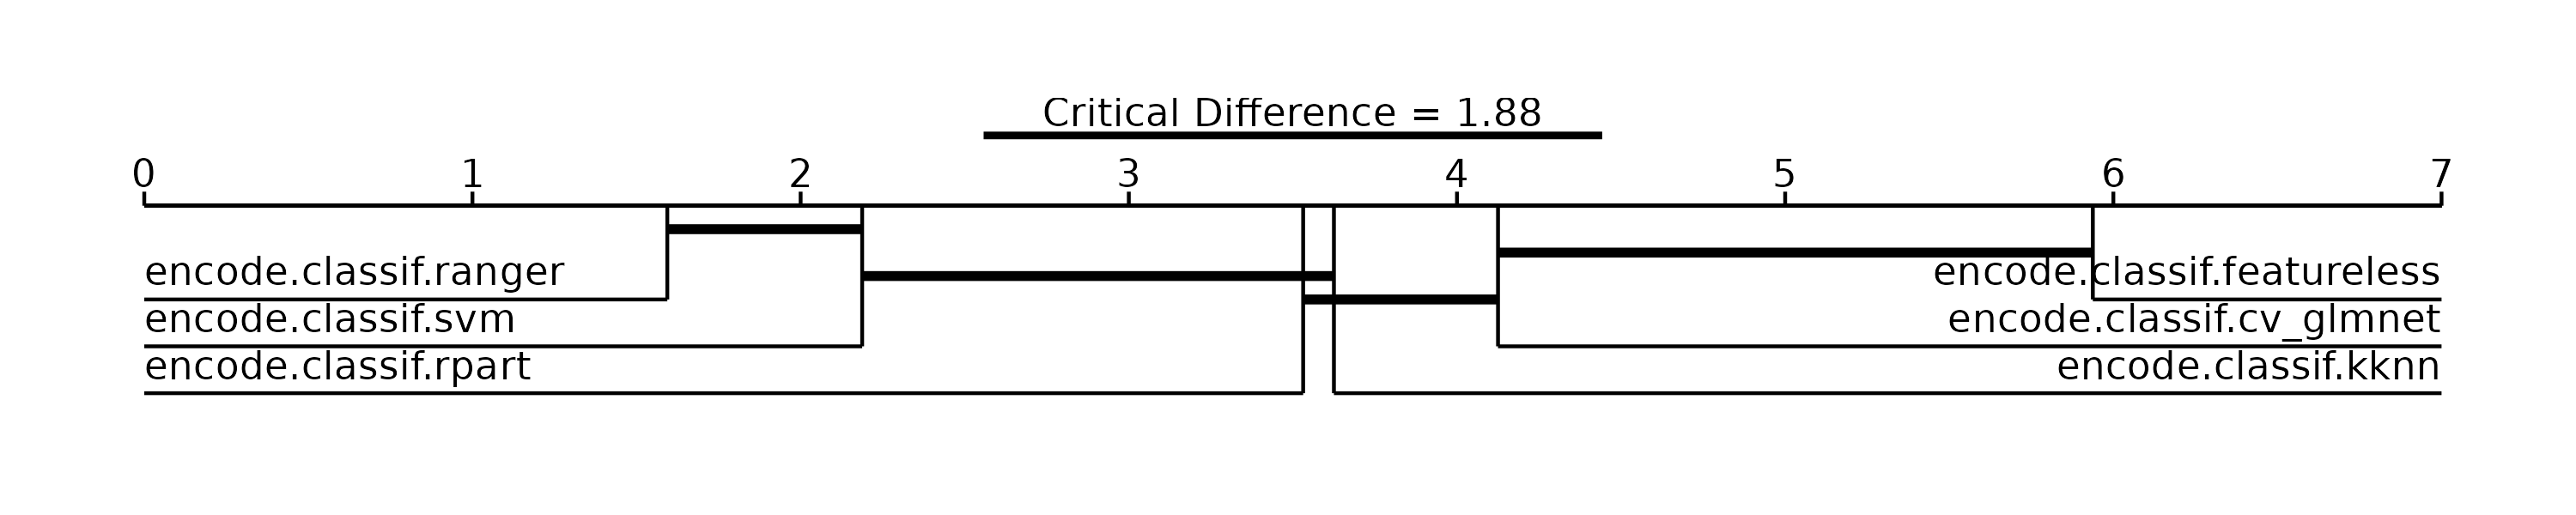
\includegraphics[width = 1.3\textwidth]{figure/crit_diff_plot.png}
\end{frame}

\begin{frame}{Post-hoc Bonferroni-Dunn test}

% \textbf{Post-hoc Bonferroni-Dunn test}:

    \begin{itemize}
    \setlength\itemsep{1em}
    \item Instead of pairwise comparisons, we now compare all algorithms with one baseline algorithm (i.e., $K-1$ comparisons).
    \item The Bonferroni-Dunn test uses a similar test statistic which is standard normally distributed under $H_0$:
    $$
        T_{\text{Bonferroni-Dunn}} = \frac{\bar{R}_{.k} - \bar{R}_{.baseline}}{\sqrt{\frac{K(K+1)}{6M}}}
    $$
    % \item The test statistic is the same as before:
    % $$
    %     T_{\text{Bonferroni-Dunn}} = \frac{\bar{R}_{.k_1} - \bar{R}_{.k_{\text{baseline}}}}{\sqrt{\frac{K(K+1)}{6M}}}
    % $$
    % \item
    % The performances of $j_1$ and $j_2$ differ significantly if $|q| > q_{\alpha}$, where the
    % .
    %Another difference between Bonferroni-Dunn Test with Nemenyi test is that total number of comparisons are 1/k of Nemenyi test.
     \item It uses the Bonferroni correction for multiple testing, so the significance level $\alpha$ is adjusted downward via the number of comparisons:
     $$
        \alpha_{\text{corrected}} = \frac{\alpha}{K - 1}
     $$
     \item For instance, $\alpha = 0.05$ is adjusted to $\alpha_{\text{corrected}} = \frac{0.05}{5} = 0.01$.
     \item Power is greater for Bonferroni-Dunn than for Nemenyi due to only comparing to a control classifier and not between all algorithms.
     % \item Generally, we want to test whether a newly proposed method is better than an existing one and thus, the Bonferroni-Dunn test is preferable in most settings.
     \end{itemize}
\end{frame}

\section{Conclusion}

\begin{frame}{Overview of different hypothesis tests}
% https://docs.google.com/presentation/d/1iiaVfeVwJJEFTTal_2dYQYOPm_WiykKBNAcryAWuLHk/edit#slide=id.p
\begin{center}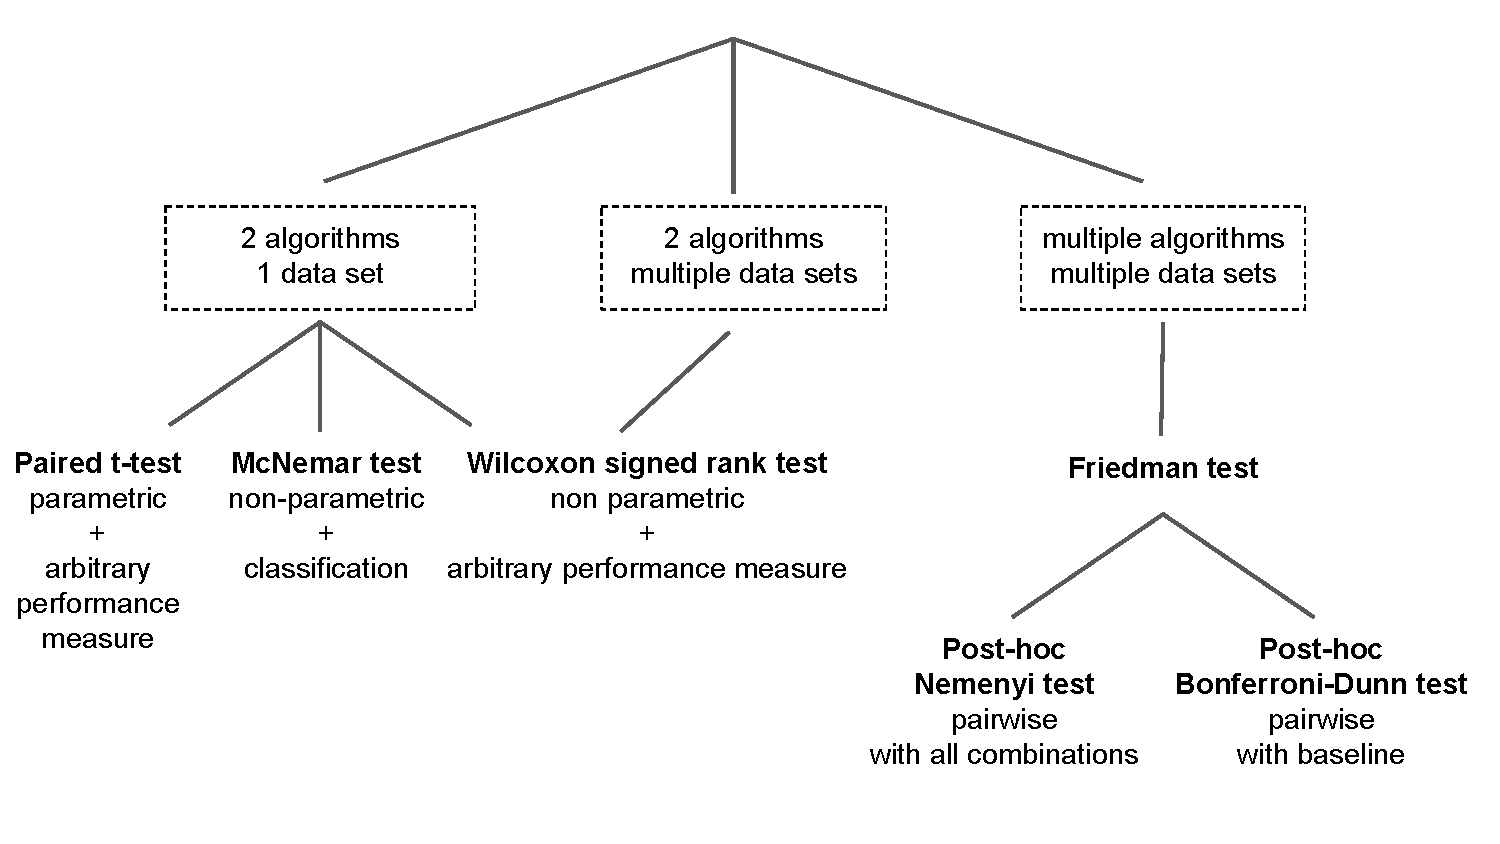
\includegraphics[width = 1\textwidth]{figure/tests.pdf} \end{center}

% \footnotesize
% {\tiny{Source: Evaluating Learning Algorithms:
% A Classification Perspective}\par}

\end{frame}


\begin{frame}{Guidelines on Hypothesis Tests}

\vfill
\begin{itemize}
    \item There is no golden standard for using hypothesis testing in performance evaluation. Often, tests are based on questionable or unverifiable assumptions or conclusions.
    \item The Wilcoxon and Friedman tests have been demonstrated to be most useful. They partially fulfil commensurability, do not assume normal distributions or homogeneity of variance, and can be applied to any evaluation metric (e.g., accuracy, error ratios).
    \item  "Tests provide certain reassurance about the validity and non-randomness of the published  results. For that to be true, they should be performed correctly and the resulting conclusions should  be drawn cautiously. On the other hand, statistical tests should not be the deciding factor for or  against publishing the work. Other merits of the proposed algorithm that are beyond the grasp of  statistical testing should also be considered and possibly even favoured over pure improvements in  predictive power." (Japkowiecz)
\end{itemize}
\vfill

\end{frame}

\begin{frame}{Guidelines on Model Selection}
    \vfill
    \begin{itemize}
        \item Know what you are optimizing $\rightarrow$ be suspicious of huge improvements
        \item Understand the difference between comparing trained models and machine learning algorithms
        \item Your machine learning metric is only a proxy for your business metric $\rightarrow$ gains might not materialize in real-world improvement
        \item Non-i.i.d. data require special treatment
        \item Multi-objective model selection and tests are still an open area of research
    \end{itemize}
    \vfill
\end{frame}


\endlecture
\end{document}
